\documentclass{article} % For LaTeX2e
\usepackage{nips11submit_e,times}
%\documentstyle[nips10submit_09,times,art10]{article} % For LaTeX 2.09

\title{Multi-Scale Language Modeling with InDel Likelihood}

\author{
Nicholas Bartlett and Frank Wood\\
Department of Statistics\\
Columbia University\\
New York, NY 10027 \\
\texttt{\{bartlett, fwood\}@stat.columbia.edu}
%\And
%Frank  Wood\\
%Columbia University\\
%Address \\
%\texttt{email} \\
%\AND
%Coauthor \\
%Affiliation \\
%Address \\
%\texttt{email} \\
%\And
%Coauthor \\
%Affiliation \\
%Address \\
%\texttt{email} \\
%\And
%Coauthor \\
%Affiliation \\
%Address \\
%\texttt{email} \\
%(if needed)\\
}

% The \author macro works with any number of authors. There are two commands
% used to separate the names and addresses of multiple authors: \And and \AND.
%
% Using \And between authors leaves it to \LaTeX{} to determine where to break
% the lines. Using \AND forces a linebreak at that point. So, if \LaTeX{}
% puts 3 of 4 authors names on the first line, and the last on the second
% line, try using \AND instead of \And before the third author name.

\newcommand{\fix}{\marginpar{FIX}}
\newcommand{\new}{\marginpar{NEW}}

%\nipsfinalcopy % Uncomment for camera-ready version

\begin{document}

\maketitle

\newcommand{\G}{\mathcal{G}}
\newcommand{\PY}{\mathcal{P}\mathcal{Y}}
\newcommand{\ES}{\mathcal{E}\mathcal{S}}
\newcommand{\likelihood}{\mathcal{L}}
\newcommand{\HPY}{\mathcal{H}\PY}


% !TEX root = deplump.tex
\subsection*{Abstract}


% !TEX root = main.tex
\section{Introduction}
\label{section_introduction}

Predictive models are all about doing as much as you can with as little data and computation as possible.  If sufficient for application purposes, resorting to simple models is often effective.  

Richly expressive models require   

Bayesian approaches to prediction dictate tying and sharing parameters, often through hierarchies and so forth. 

Cite 

Related work on multiscale language modeling
\citep{Goldwater2009,Mochihashi2009}

Related work on transformed Dirchlet processes and HDP's with random effects.
\citep{Sudderth2005,Kim2007,Hoffman2009,}
% !TEX root = deplump.tex
\section{Methodology}
\label{section:methodology}
\newcommand{\PY}{\ensuremath{\mathcal{P}\mathcal{Y}}}

\subsection{Review}

Note that a probability distribution $P$ over sequences can be factorized as $P(S = [s_0, s_1, \ldots, s_m]) = P(s_0)P_{[s_0]}(s_1)P_{[s_0,s_1]}(s_2) \ldots P_{[s_0,s_1,\ldots,s_{m-1}]}(s_m)$, where $P_u(s) = P(s | u)$.  The sequence memoizer jointly models these conditional distributions using a hierarchical Bayesian framework.  The hierarchy used to define the model makes use of the Pitman-Yor distribution over distributions. If $P \sim \PY(d,c,G)$ then we say $P$ follows a Pitman-Yor distribution with discount parameter $d$, concentration parameter $c$ and mean distribution $G$.  The mean distribution $G$ can be understood as the average $P$ resulting from this distribution, i.e. $\mathbb{E}(P(S)) = G(S)$ for $S \in \Sigma^{+}$.  The discount parameter is a real value between 0 and 1.  If the discount is close to 1 it is an indication that $P$ is likely to be very close to $G$; d close to 0 indicates $P$ may vary significantly from $G$.  In the sequence memoizer the concentration parameters are restricted to 0 and will be omitted from the remaining discussion. If we define the operator $\sigma$ on discrete sequences as $\sigma([s_0, s_1, \ldots, s_m]) = [s_1,s_2, \ldots, s_m])$ then we can write the sequence memoizer model as 
%
\begin{eqnarray*}
	P_{[ ]} &\sim& \PY(d_0,0,\mathcal{U}(\Sigma))\\
	P_{u} &\sim& \PY(d_{|u|}, 0, P_{\sigma(u)})
\end{eqnarray*}
\noindent where $\mathcal{U}(\Sigma)$ is the uniform distribution over $\Sigma$.  The hierarchy used in the model smoothes each conditional distribution $P_u$ towards a related, more general distribution $P_{\sigma(u)}$.  Intuitively the hierarchy indicates that the most recent context is the most informative for modeling the conditional distributions.

Inference in the model is performed using a compressed representation in which only two counts for each symbol need to be maintained for a set of conditional distributions which grows linearly in the length of the sequence.  Bayesian inference is typically performed by averaging over the posterior distributions of parameters, but \cite{Gasthaus2010} demonstrate that using a single particle approximation yields excellent empirical results. \cite{Bartlett2010}  show that by making some independence assumptions the approximation can be extended to facilitate a constant space inference procedure without much loss in  empirical performance.

\subsection{Approximation}

The counts that are maintained in the inference procedure grow at a sublinear rate, but are not bounded above.  Unfortunately the computation required to update the model as new data is observed grows as a linear function of these counts.  Therefore, to make the algorithm computationally tractable to streaming sequence, the total count for each conditional distribution must be bounded above.  This further approximation then caps the computation time for each model update at some reasonable level and does not have effect on empirical performance.  
% !TEX root = deplump.tex
\section{Experiments}
\label{sec:experiments}

As the performance of batch deplump was established relative to other lossless compressors for a variety of datatypes in \citep{Gasthaus2010}, we focus our experiments on establishing a) that the approximations to inference in the sequence memoizer combined in this paper in order to make deplump a streaming compressor do not significantly adversely affect compression performance, b) that the resulting compressor can indeed compress extremely long sequences as the asymptotic guarantees would suggest it should, and c) what settings of the approximation parameters produce the best compression performance.

Before testing the algorithm on streaming corpus we compared the algorithm to batch deplump.  We compressed the 100Mb Wikipedia corpus used for the Hutter Prize \citep{Hutter2006} using the streaming variant of deplump with $L = 10^{7}$ and $D = 16$ and found it gives a compression ratio of 4.78.  Using batch deplump gives a compression ratio of 4.82 \citep{Gasthaus2010}, while running batch deplump repeatedly on the 5Mb subsections of the corpus reduces the compression ratio to 4.25.  These results demonstrate that the approximations made for streaming deplump give it a significant advantage over compressing the file in chunks and have very little negative effect when compared to the full model.

All of the experiments included in this paper use a complete Wikipedia text content dump \citep{Wikipedia} as a test corpus (26.8Gb uncompressed, 7.8Gb gziped and ??Gb paq9a'ed, each with default parameters, and 3.9Gb deplumped).  To establish what approximation parameters produce the best compression results we first ran streaming deplump on the first 100Mb section of the corpus limiting the depth to two different values ($D=16$ and $D=1024$) with a fixed limit on the number of nodes in the tree ($L=10^6$).  We observed that in both cases only very few nodes had high total counts ($c > 8,192$) suggesting that it might be possible to set the count upper bound to a relatively low value ($k= 8,192$) without significant compression performance degradation.  %That compression performance should not be affected by a reasonable count bound follows intuitively from the fact that in byte sequences $|\Sigma| = 256$ and setting $k=10,000$ is similar in effect to using 10,000 observations to estimate a 256 element discrete distribution.  
To ensure that compression performance did in fact not suffer, we compressed ten 100Mb subsections of the corpus (sampled randomly with replacement) for multiple values of $k$ between 128 and 32,768 (fixing $L=10^6$ and $D=16$).  We observed that average compression performance varied insignificantly over $k$ for $2^7 \leq k \leq s^{15}$.

 In each of the following experiments, subsections of the corpus were sampled with replacement.  In the first experiment the sampled subsections were all of size 100Mb, while in the second the sampled subsections varied in length.  In the first experiment, the interplay between limiting the number of nodes in the tree and restricting the depth of the tree was explored (results for which are shown in Figure~\ref{fig:varying_depths}).  Here $k$ was set to 8,192, while $L$ and the depth of the tree $D$ were varied as indicated in the figure.  In the second experiment, the interplay between stream length and node limit was explored (Figure~\ref{fig:varying_stream_length}).  In this experiment $k$ remained fixed at the same value and the depth was set to $D=16$ while $L$ varied as shown in the figure.  

Figure~\ref{fig:varying_depths} indicates that compression performance becomes essentially indistinguishable for depth restrictions greater than $D=10$.  However, this figure also suggests that compression performance almost always improves as a function of the number of nodes in the tree for depths 6 and greater.  Figure~\ref{fig:varying_stream_length} illustrates that the algorithm not only scales to very long sequences, but average compression performance continues to improve as the sequence grows.  Using a large value of $L$ appears to be beneficial for very long sequences.

\begin{figure*}[t] 
	\begin{center}
		\scalebox{.6}{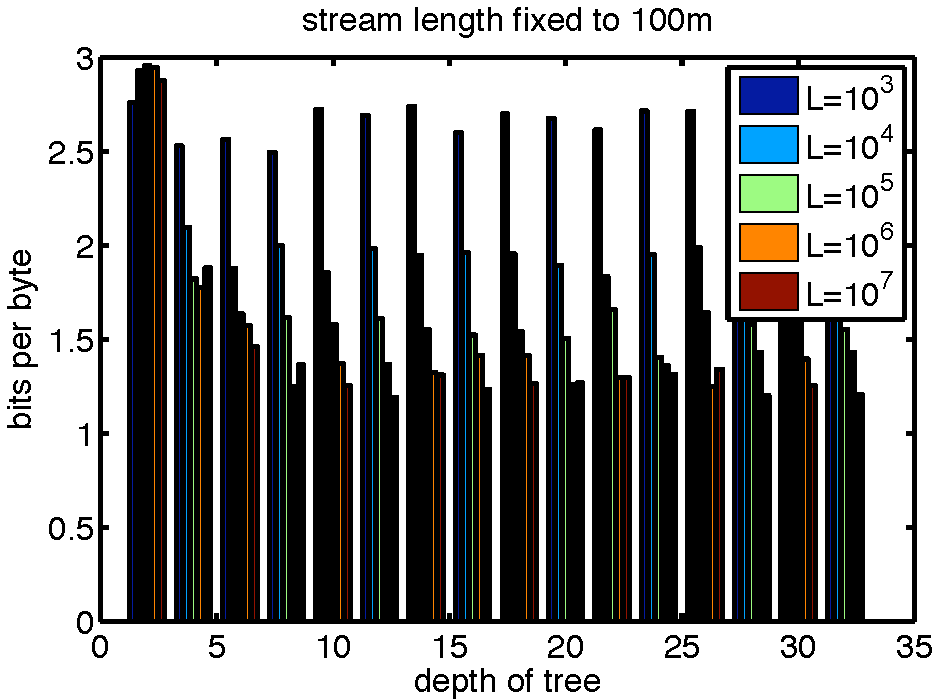
\includegraphics{figs/varying_depths.pdf}} % [clip=true, viewport= 1in 1in 9in 9in]
		\caption{Performance averaged over 10 random sections  100Mb sections of the corpus for varying fixed depths and number of allowable nodes ($L$) }
		\label{fig:varying_depths}
	\end{center} 
\end{figure*} 

%\begin{figure*}[t] 
%	\begin{center}
%		\scalebox{.6}{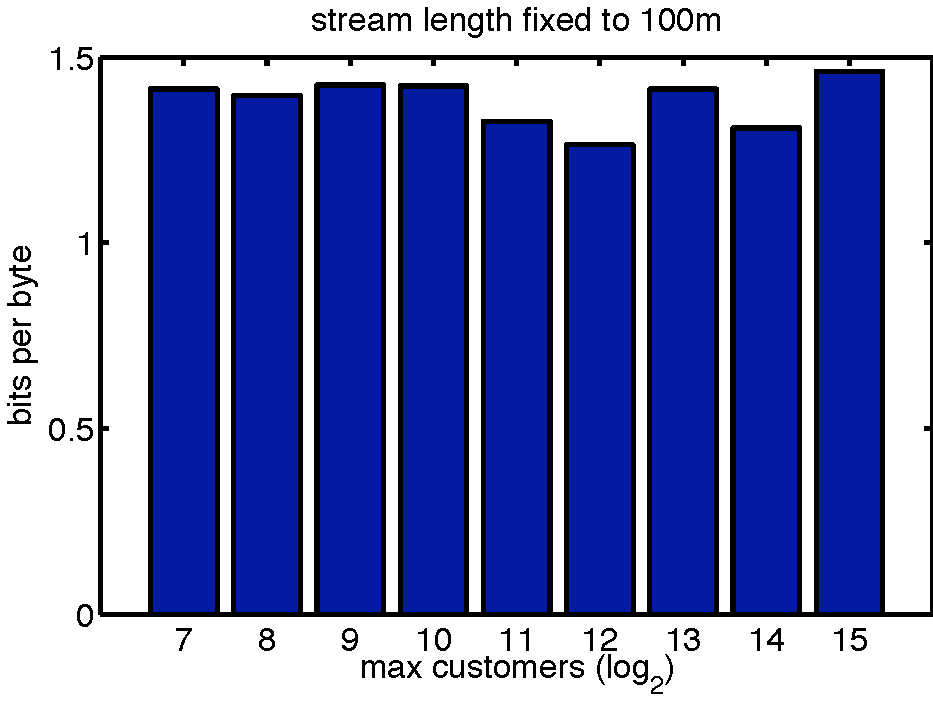
\includegraphics{figs/varying_max_customers.pdf}} % [clip=true, viewport= 1in 1in 9in 9in]
%		\caption{Performance for varying max allowable customers $k$.}
%		\label{fig: varying_max_customers}
%	\end{center} 
%\end{figure*} 

\begin{figure*}[t] 
	\begin{center}
		\scalebox{.6}{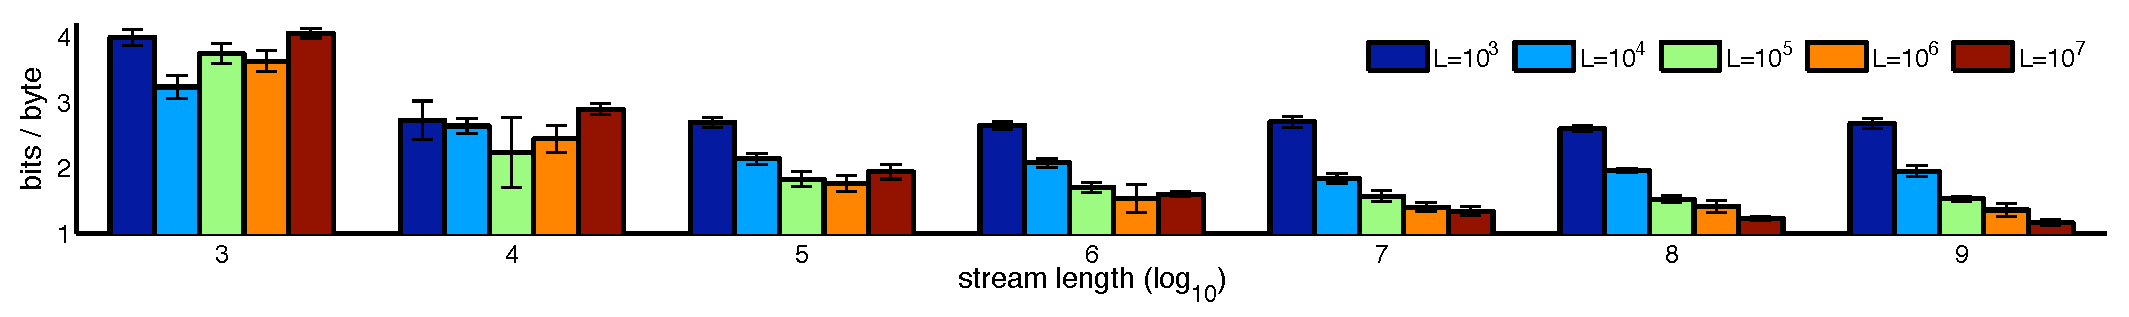
\includegraphics{figs/varying_stream_length.pdf}} % [clip=true, viewport= 1in 1in 9in 9in]
		\caption{Performance for varying stream lengths and number of allowable nodes ($L$).}
		\label{fig:varying_stream_length}
	\end{center} 
\end{figure*} 


%\begin{figure*}[t] 
%	\begin{center}
%		\scalebox{1}{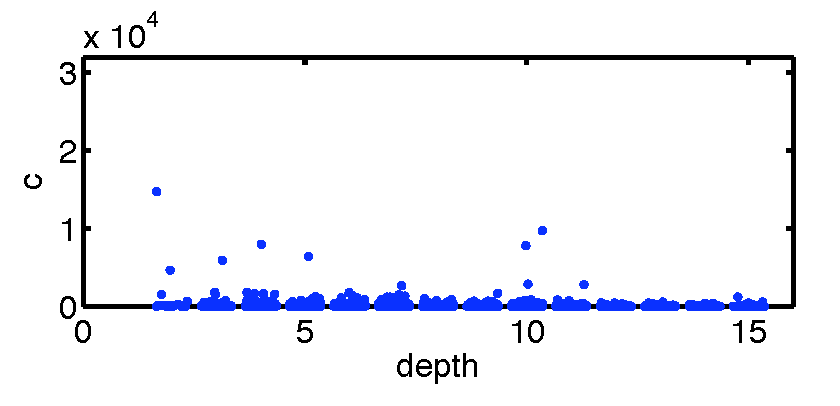
\includegraphics{figs/scatter_16.pdf}} % [clip=true, viewport= 1in 1in 9in 9in]
%		\caption{Scatter plots to explore the relationship between the depth of a node and the total count}
%		\label{fig:restaurant_plots}
%	\end{center} 
%\end{figure*} 

%\begin{figure*}[t] 
%	\begin{center}
%		\scalebox{1}{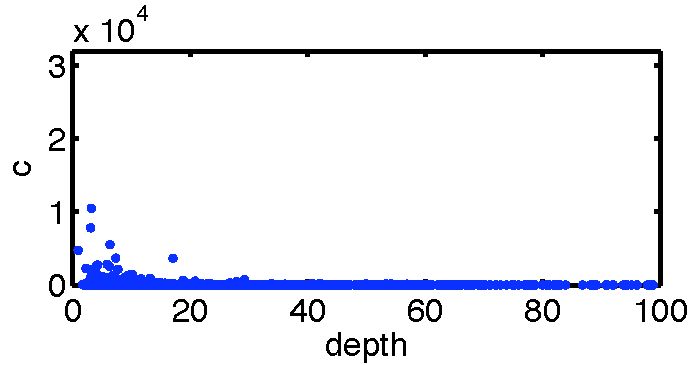
\includegraphics{figs/scatter_1024.pdf}} % [clip=true, viewport= 1in 1in 9in 9in]
%		\caption{Scatter plots to explore the relationship between the depth of a node and the total count}
%		\label{fig:restaurant_plots}
%	\end{center} 
%\end{figure*} 

% !TEX root = main.tex
\section{Discussion}
\label{section_discussion}

Things to consider: 

1) Scaling to phrases.
2) Making the spelling correction parameterization context dependent.


\begin{small}
\bibliographystyle{plainnat}
\bibliography{../../uber} 
\end{small}

\end{document}
